% Chapter Template

\chapter{An approach to VAD using PEFAC} % Main chapter title

\label{Chapter5} % Change X to a consecutive number; for referencing this chapter elsewhere, use \ref{ChapterX}

\lhead{Chapter 5. \emph{An approach to VAD using PEFAC}} % Change X to a consecutive number; this is for the header on each page - perhaps a shortened title

%----------------------------------------------------------------------------------------
%	SECTION 1 - PEFAC pitch tracker
%----------------------------------------------------------------------------------------

\section{PEFAC pitch tracker}

PEFAC pitch tracker \cite{PEFAC} is one of the recently published, robust pitch tracking algorithms which has been reported to achieve good results even at negative signal to noise ratios. Apart from calculating the pitch estimate as its primary output, it has also been designed to estimate the probability of a given frame \emph{being voiced} which is essentially a voiced speech activity detector. This value can be used to detect the voiced parts of a speech utterance by simple thresholding. Subsequent application of a hang-over scheme from Chapter \ref{Chapter3} should help in detecting the unvoiced segments. A combination of a thresholding stage and the hang-over scheme therefore creates a complete Voice Activity Detector.

The rest of this chapter is organised as follows. Firstly, an overview of PEFAC is presented. Then, the proposed approach to VAD is described in more detail, implemented and evaluated against LTSD, which was the best performing VAD from Chapter \ref{Chapter4}. The experimental set-up for evaluation of PEFAC as VAD is the same as described in Chapter \ref{Chapter3}.

%----------------------------------------------------------------------------------------
%	SUBSECTION 1 - PEFAC algorithm description
%----------------------------------------------------------------------------------------

\subsection{PEFAC algorithm description}

A detailed description of PEFAC is available in \cite{PEFAC}. The algorithm can however be summarised in the following steps:
\begin{enumerate}
\item Transform the input signal to the power spectrum domain using short-time Fourier transform
\item Interpolate the periodogram of each frame onto a log-spaced frequency grid
\item Calculate the normalized periodogram
\item Convolve the normalized periodogram with a comb filter in order to enhance speech harmonics and attenuate the noise
\item Select the three highest peaks in the feasible range as the initial pitch candidates
\item Estimate the probability of a frame being voiced
\item Use dynamic programming to identify the final pitch estimate
\end{enumerate}

The probability of a frame being voiced is based on two features:
\begin{enumerate}
\item The log-mean power of a frame $L_t = \log E_t$ such that $E_t = \frac{1}{Q} \sum_{n=1}^{Q} Y_t(q_i)$ where $Q$ is the number of frequency bins, $Y_t(q)$ is the normalized log-frequency periodogram. Using the log-mean power is justified since voiced speech typically contains most energy contained in a complete speech utterance and its mean power is therefore higher than that of unvoiced speech
\item The ratio of the sum of the highest three peaks in the spectrum convolved with the comb filter to $E_t$. Voiced speech contains most of its power in the harmonic bins therefore using this measure as a second feature is justified
\end{enumerate}

%----------------------------------------------------------------------------------------
%	SECTION 2
%----------------------------------------------------------------------------------------

\section{The proposed approach}

The proposed approach is relatively simple. PEFAC returns the probability of the current frame being voiced in a typical manner, i.e. as a number in the range 0 to 1. This can easily be thresholded and the voiced frames can be identified at this step. As stated numerously in the previous chapters, the voiced frames are typically surrounded by the unvoiced ones, hence application of the hang-over scheme from Section \ref{sec:hang} will help to detect them. On average, this approach should perform well in detection of both the voiced as well as unvoiced phonemes which is the aim of a complete Voice Activity Detector.

%----------------------------------------------------------------------------------------
%	SECTION 3 - Evaluation results
%----------------------------------------------------------------------------------------

\section{Evaluation results}

The proposed approach has been implemented, evaluated and compared with the LTSD VAD. In all experiments, the hang-over scheme (Section \ref{sec:hang}) has been applied to both algorithms. The evaluation of PEFAC without it does not make much sense, since by design it does not detect unvoiced phonemes and do they need to be identified by a secondary method. Other than that, the evaluation metrics are the same as in Chapter \ref{Chapter4}, namely the ROC curves and speech/non-speech hit rates with a fixed threshold.

%----------------------------------------------------------------------------------------
%	SUBSECTION 1 - ROC curves
%----------------------------------------------------------------------------------------

\subsection{ROC curves}

The ROC curves for PEFAC and LTSD for all six noise types and two SNR levels (-5 dB and -10 dB) are presented in Figures \ref{fig:pefacm5} and \ref{fig:pefacm10}. For the white, car and opsroom noises, the performance of both algorithms seems to be comparable. PEFAC clearly underperforms LTSD in the babble and spchspect noises, which is expected to some extent, since being primarily a pitch tracker, the babble noise is probably the most difficult noise in which such algorithm might operate. Interestingly, PEFAC is far superior to LTSD in thr factory noise and its performance is much better in both SNR levels.

\begin{figure}[htbp]
	\centering
		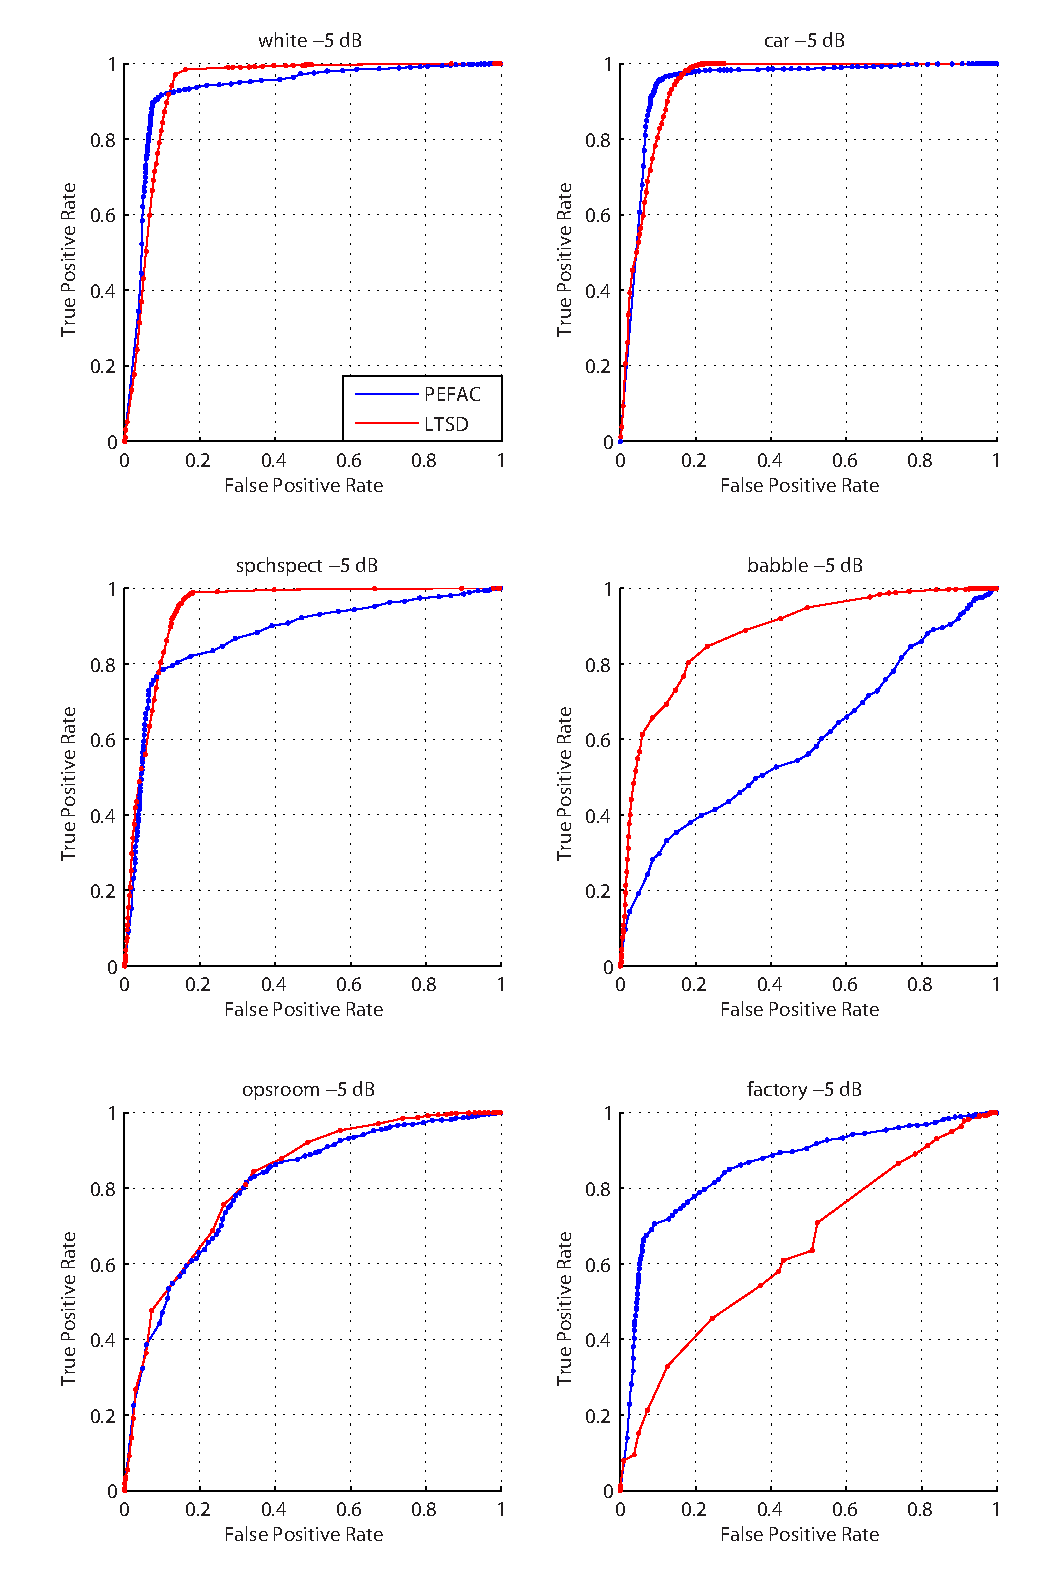
\includegraphics[width=1.0\columnwidth]{Figures/Chapter5/pefacm5.pdf}
		\rule{37em}{0.5pt}
	\caption[ROC curves of PEFAC and LTSD \emph{with} hang-over under -5 dB SNR]{ROC curves of PEFAC and LTSD \emph{with} hang-over under -5 dB SNR}
	\label{fig:pefacm5}
\end{figure}

\begin{figure}[htbp]
	\centering
		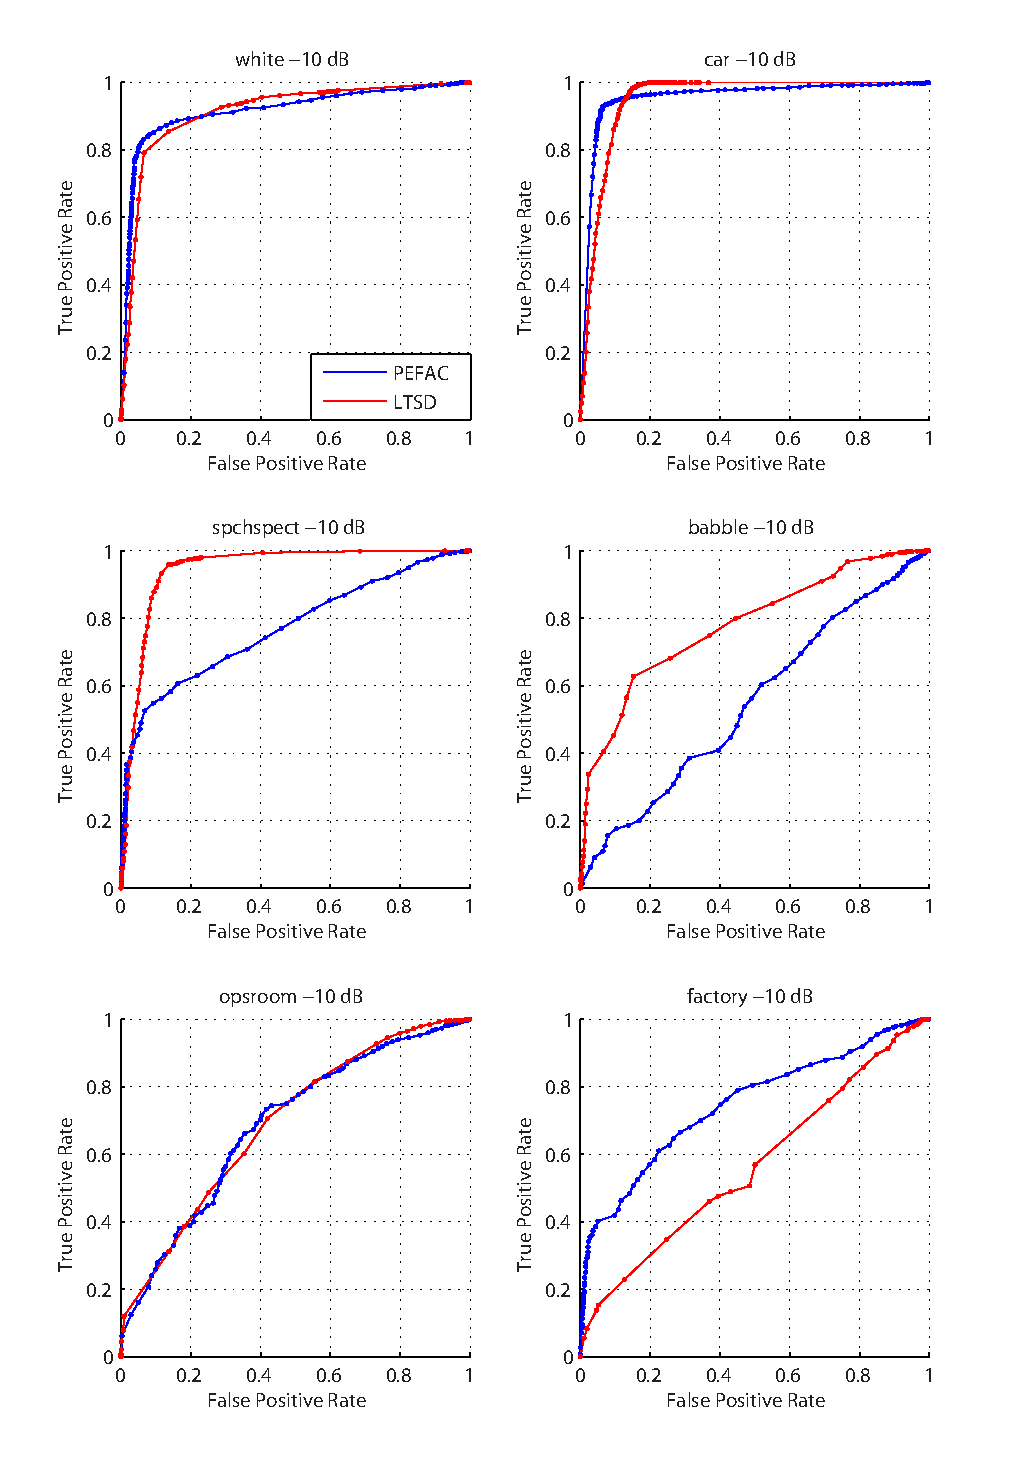
\includegraphics[width=1.0\columnwidth]{Figures/Chapter5/pefacm10.pdf}
		\rule{37em}{0.5pt}
	\caption[ROC curves of PEFAC and LTSD \emph{with} hang-over under -10 dB SNR]{ROC curves of PEFAC and LTSD \emph{with} hang-over under -10 dB SNR}
	\label{fig:pefacm10}
\end{figure}

%----------------------------------------------------------------------------------------
%	SUBSECTION 2 - Speech/non-speech hit rates
%----------------------------------------------------------------------------------------

\subsection{Speech/non-speech hit rates}

The speech/non-speech hit rates with two fixed thresholds (0.60 and 0.55 respectively) are presented in Figures \ref{fig:pefacSNR60} and \ref{fig:pefacSNR55}\footnote{The threshold for PEFAC in Figure \ref{fig:pefacSNR60} is higher than in \ref{fig:pefacSNR55} therefore a lower speech hit rate but a higher non-speech hit rate. The thresholds are 0.60 and 0.55 respectively.}. Interestingly, for both threshold values PEFAC overperforms LTSD at low and very low SNRs i.e. in the range 0 to -15 dB. For the higher value of the fixed threshold (Figure \ref{fig:pefacSNR60}) PEFAC's performance is clearly better even in both speech and non-speech metrics while for the lower threshold, the non-speech hit rate at the low SNRs is very similar for both algorithms.

There is a slight disadvantage in the performance of PEFAC in the speech hit rate at the high SNR levels (20 dB to 5 dB). The exact position of the errors has been investigated visually by examining plots of the test set overlayed with the reference labels and VAD decisions. It has been determined that the vast majority of PEFAC's speech as noise misclassifications appear at the very endings of the utterances. This is visualised in Figure \ref{fig:clipping} where such errors are labelled as BEC - back end clipping. The errors which do appear are very short, with the length of 1-2 frames and hence can be described as minor. There are virtually no MSC (midspeech clipping) errors, which are more severe, for both LTSD and PEFAC at high SNRs and only a small number of FEC (front end clipping) errors.

\begin{figure}[htbp]
	\centering
		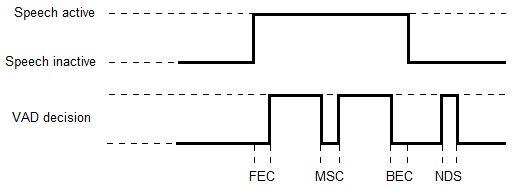
\includegraphics[width=1.0\columnwidth]{Figures/Chapter5/clipping.png}
		\rule{37em}{0.5pt}
	\caption[Types of misclassifications in VAD]{Types of misclassifications in VAD. FEC - front end clipping, MSC - midspeech clipping, BEC - back end clipping, NDS - noise detected as speech}
	\label{fig:clipping}
\end{figure}

\vfill

\begin{figure}[htbp]
	\centering
		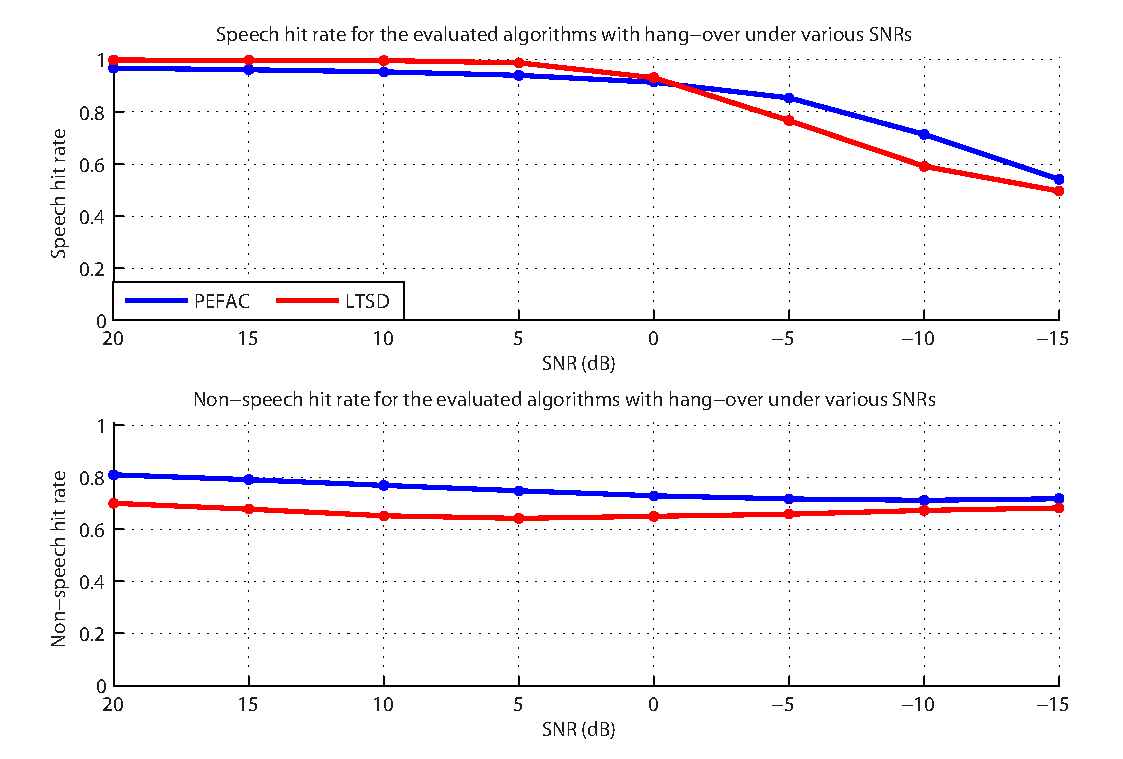
\includegraphics[width=0.9\columnwidth]{Figures/Chapter5/pefacSNR60bold.pdf}
		\rule{37em}{0.5pt}
	\caption[Speech/non-speech hit rates for PEFAC (threshold 0.60) and LTSD under different SNRs]{Speech/non-speech hit rates for PEFAC (threshold 0.60) and LTSD under different SNRs}
	\label{fig:pefacSNR60}
\end{figure}

\clearpage

\begin{figure}[htbp]
	\centering
		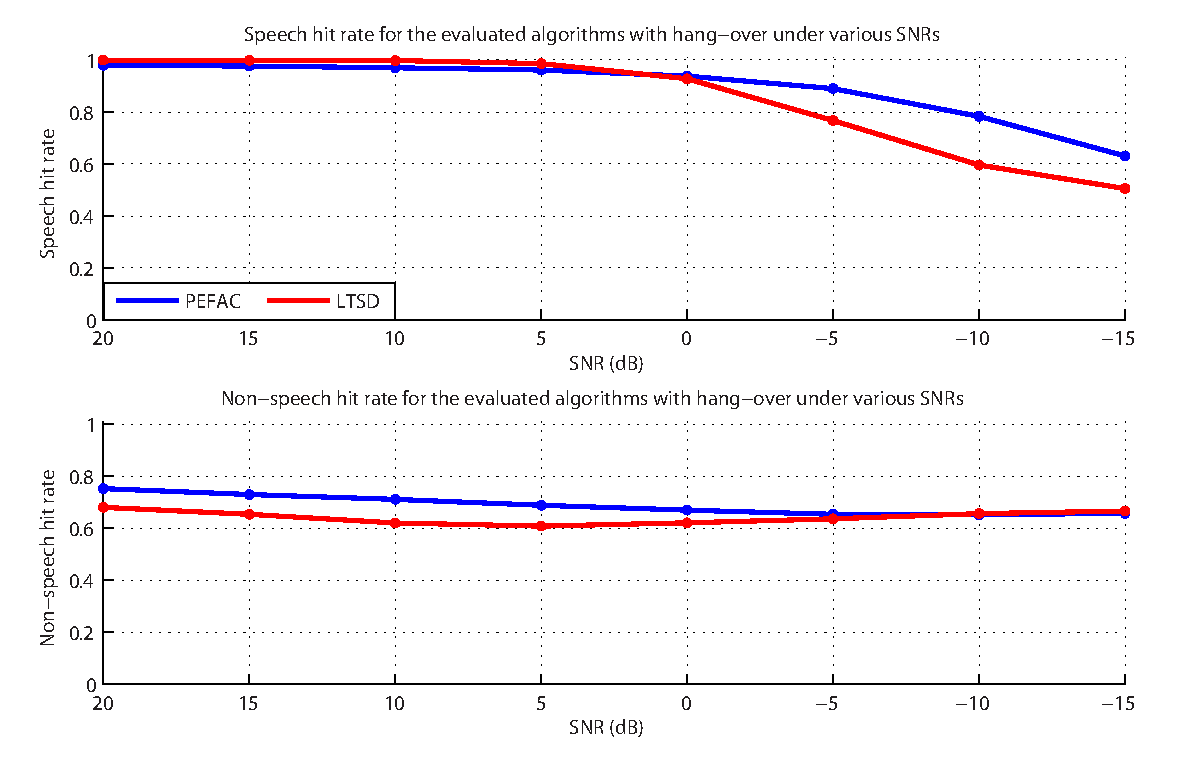
\includegraphics[width=0.9\columnwidth]{Figures/Chapter5/pefacSNR55bold.pdf}
		\rule{37em}{0.5pt}
	\caption[Speech/non-speech hit rates for PEFAC (threshold 0.55) and LTSD under different SNRs]{Speech/non-speech hit rates for PEFAC (threshold 0.55) and LTSD under different SNRs}
	\label{fig:pefacSNR55}
\end{figure}

%----------------------------------------------------------------------------------------
%	SECTION 4 - The effect of hang-over parameters
%----------------------------------------------------------------------------------------

\section{The effect of hang-over parameters}

The fact that most speech misclassifications are BEC errors indicates a hypothesis that the differences in the performance of both algorithms at the high SNR levels could be reduced by careful calibration of the hang-over parameters and the frame length. In particular, the parameters ($L_s$ and $L_m$ as in Algorithm \ref{algo:hangover}) with which the previous evaluation has been performed are not large enough to extend the initial VAD decisions to capture all beginnings and endings of the speech utterances. In order to confirm the hypothesis, an experimentation with various different parameter values has been performed and the speech/non-speech hit rates have been examined. It transpired that by reducing the frame length\footnote{The frame length has been reduced from 50 ms to 25 ms.} and adjusting the other parameters appropriately\footnote{The new parameter velues are $B=14$, $S_p=3$, $S_l=5$, $L_s=18$ and $L_m=25$}, the performance of both algorithms can be rendered almost equal at the high SNR levels with PEFAC still outperforming LTSD at the low SNRs. Figure \ref{fig:diffhangpars} presents the result of the new evaluation.

\begin{figure}[htbp]
	\centering
		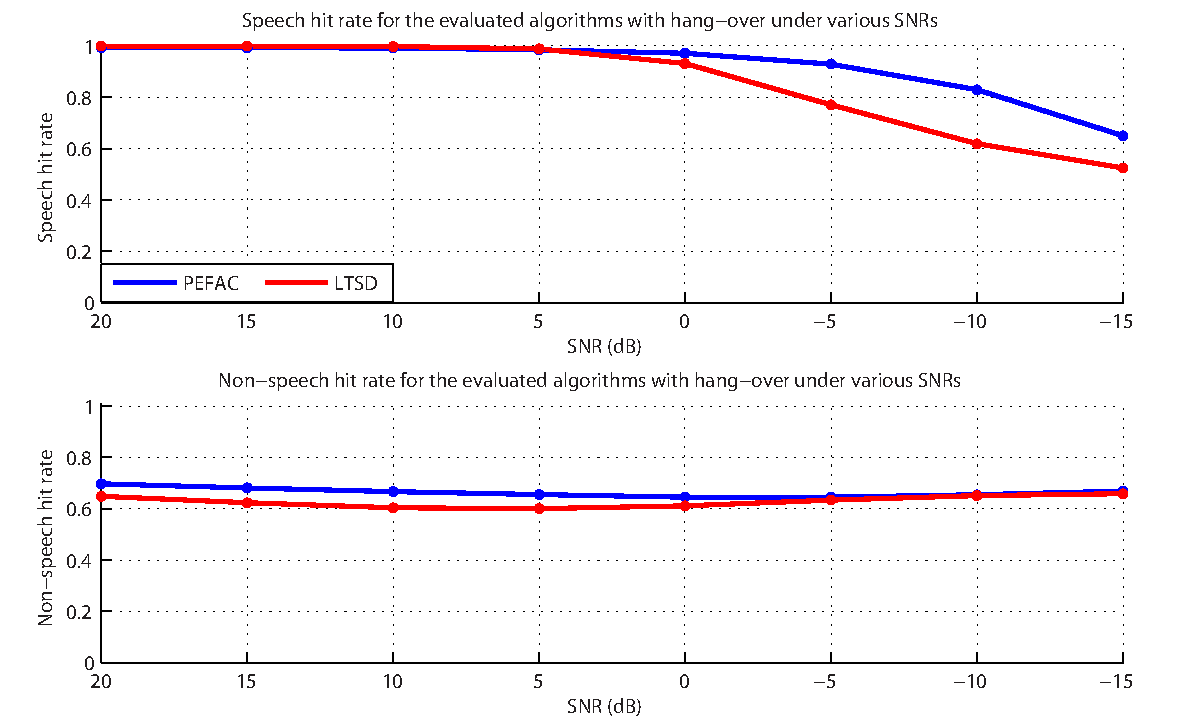
\includegraphics[width=0.9\columnwidth]{Figures/Chapter5/diffhangpars.pdf}
		\rule{37em}{0.5pt}
	\caption[Speech/non-speech hit rates for PEFAC (threshold 0.60) and LTSD with adjusted hang-over parameters]{Speech/non-speech hit rates for PEFAC (threshold 0.60) and LTSD with adjusted hang-over parameters}
	\label{fig:diffhangpars}
\end{figure}

%----------------------------------------------------------------------------------------
%	SECTION 5 - Summary
%----------------------------------------------------------------------------------------

\section{Summary}

The average performance of PEFAC is better than LTSD's at the very high SNR levels (-5 to -15 dB). This performance gain comes mostly from the much better operation in the factory noise and the fact that the best performance of PEFAC in all six noise types is achieved at similar threshold values (around 0.6) while for the LTSD algorithm the threshold values vary significantly between different noise types. Therefore, it can be concluded that PEFAC should be considered for applications which have to deal with varying conditions and high noise levels.